\section{Introduction}

% 智能家居是物联网 (IoT) 的一个重要应用,在寻求更高便利性和舒适度的用户中越来越受欢迎。智能家居的一个关键特性是自动化,它由用户定义的或预先配置的规则实现,旨在简化日常任务。
Smart homes represent a significant application of the Internet of Things (IoT), gaining increasing traction among users seeking enhanced convenience and comfort. A key feature of smart homes is automation, enabled by user-defined or pre-configured rules designed to streamline daily tasks.

% 自动化规则是智能家居实现智能化的核心。一条规则通常包含三个关键部分:触发器(Trigger)、条件(Condition)和动作(Action),简称TCA。 触发器定义了规则启动的事件;条件是对触发事件发生后执行动作的先决判断;动作为满足条件时执行的具体操作。例如,考虑以下规则:当室内温度低于24摄氏度时(触发器),且空调处于关闭状态(条件),则开启空调并将温度设置为27摄氏度(动作)。这条规则的目的是实现室内温度的自动调节。 我们可以用以下形式化的方式表示这条规则:$\langle$ \texttt{indoor temperature is below 24\celsius },\texttt{air conditioner is off },\texttt{turn on the air conditioner and set the air conditioner temperature to 27\celsius } $\rangle$。
Automation rules are at the heart of smart home intelligence. A rule typically consists of three key components: Trigger, Condition, and Action (TCA). The trigger defines the event that initiates the rule; the condition provides a prerequisite check after the trigger event occurs; and the action specifies the concrete operations to be performed if the condition is met. For instance, consider a scenario where if the indoor temperature falls below 24\celsius (trigger), and the air conditioner is off (condition), then the air conditioner is turned on and set to 27\celsius (action). This rule aims to maintain a consistent indoor temperature automatically. We can represent this rule in a formalized manner as follows: $\langle$ \texttt{indoor temperature is below 24\celsius },\texttt{air conditioner is off },\texttt{turn on the air conditioner and set the air conditioner temperature to 27\celsius } $\rangle$.

% 然而,在复杂的智能家居环境中,多条规则并发执行可能导致意料之外的后果。规则之间的相互作用可能引发冲突,进而造成严重的安全隐患。例如,图\ref{rule_conflict_example} 展示了两个可能冲突的规则。规则1:当烟雾报警器被触发时,打开消防喷淋头。规则2:当检测到漏水时,关闭水阀。如果规则1被触发,打开喷淋头,这可能会导致规则2被触发,关闭水阀,从而阻碍灭火,带来火灾风险。
However, in complex smart home system, the concurrent execution of multiple rules can lead to unintended consequences. Interactions between rules may trigger conflicts, potentially leading to serious safety hazards. For example, Figure \ref{rule_conflict_example} illustrates two potentially conflicting rules. Rule 1: When the smoke alarm is triggered, turn on the fire sprinkler. Rule 2: When a water leak is detected, close the water valve. If Rule 1 is triggered, opening the sprinkler, it may in turn trigger Rule 2, closing the water valve and thus hindering fire suppression, posing a fire risk.

\begin{figure}[htbp]
	\centering
	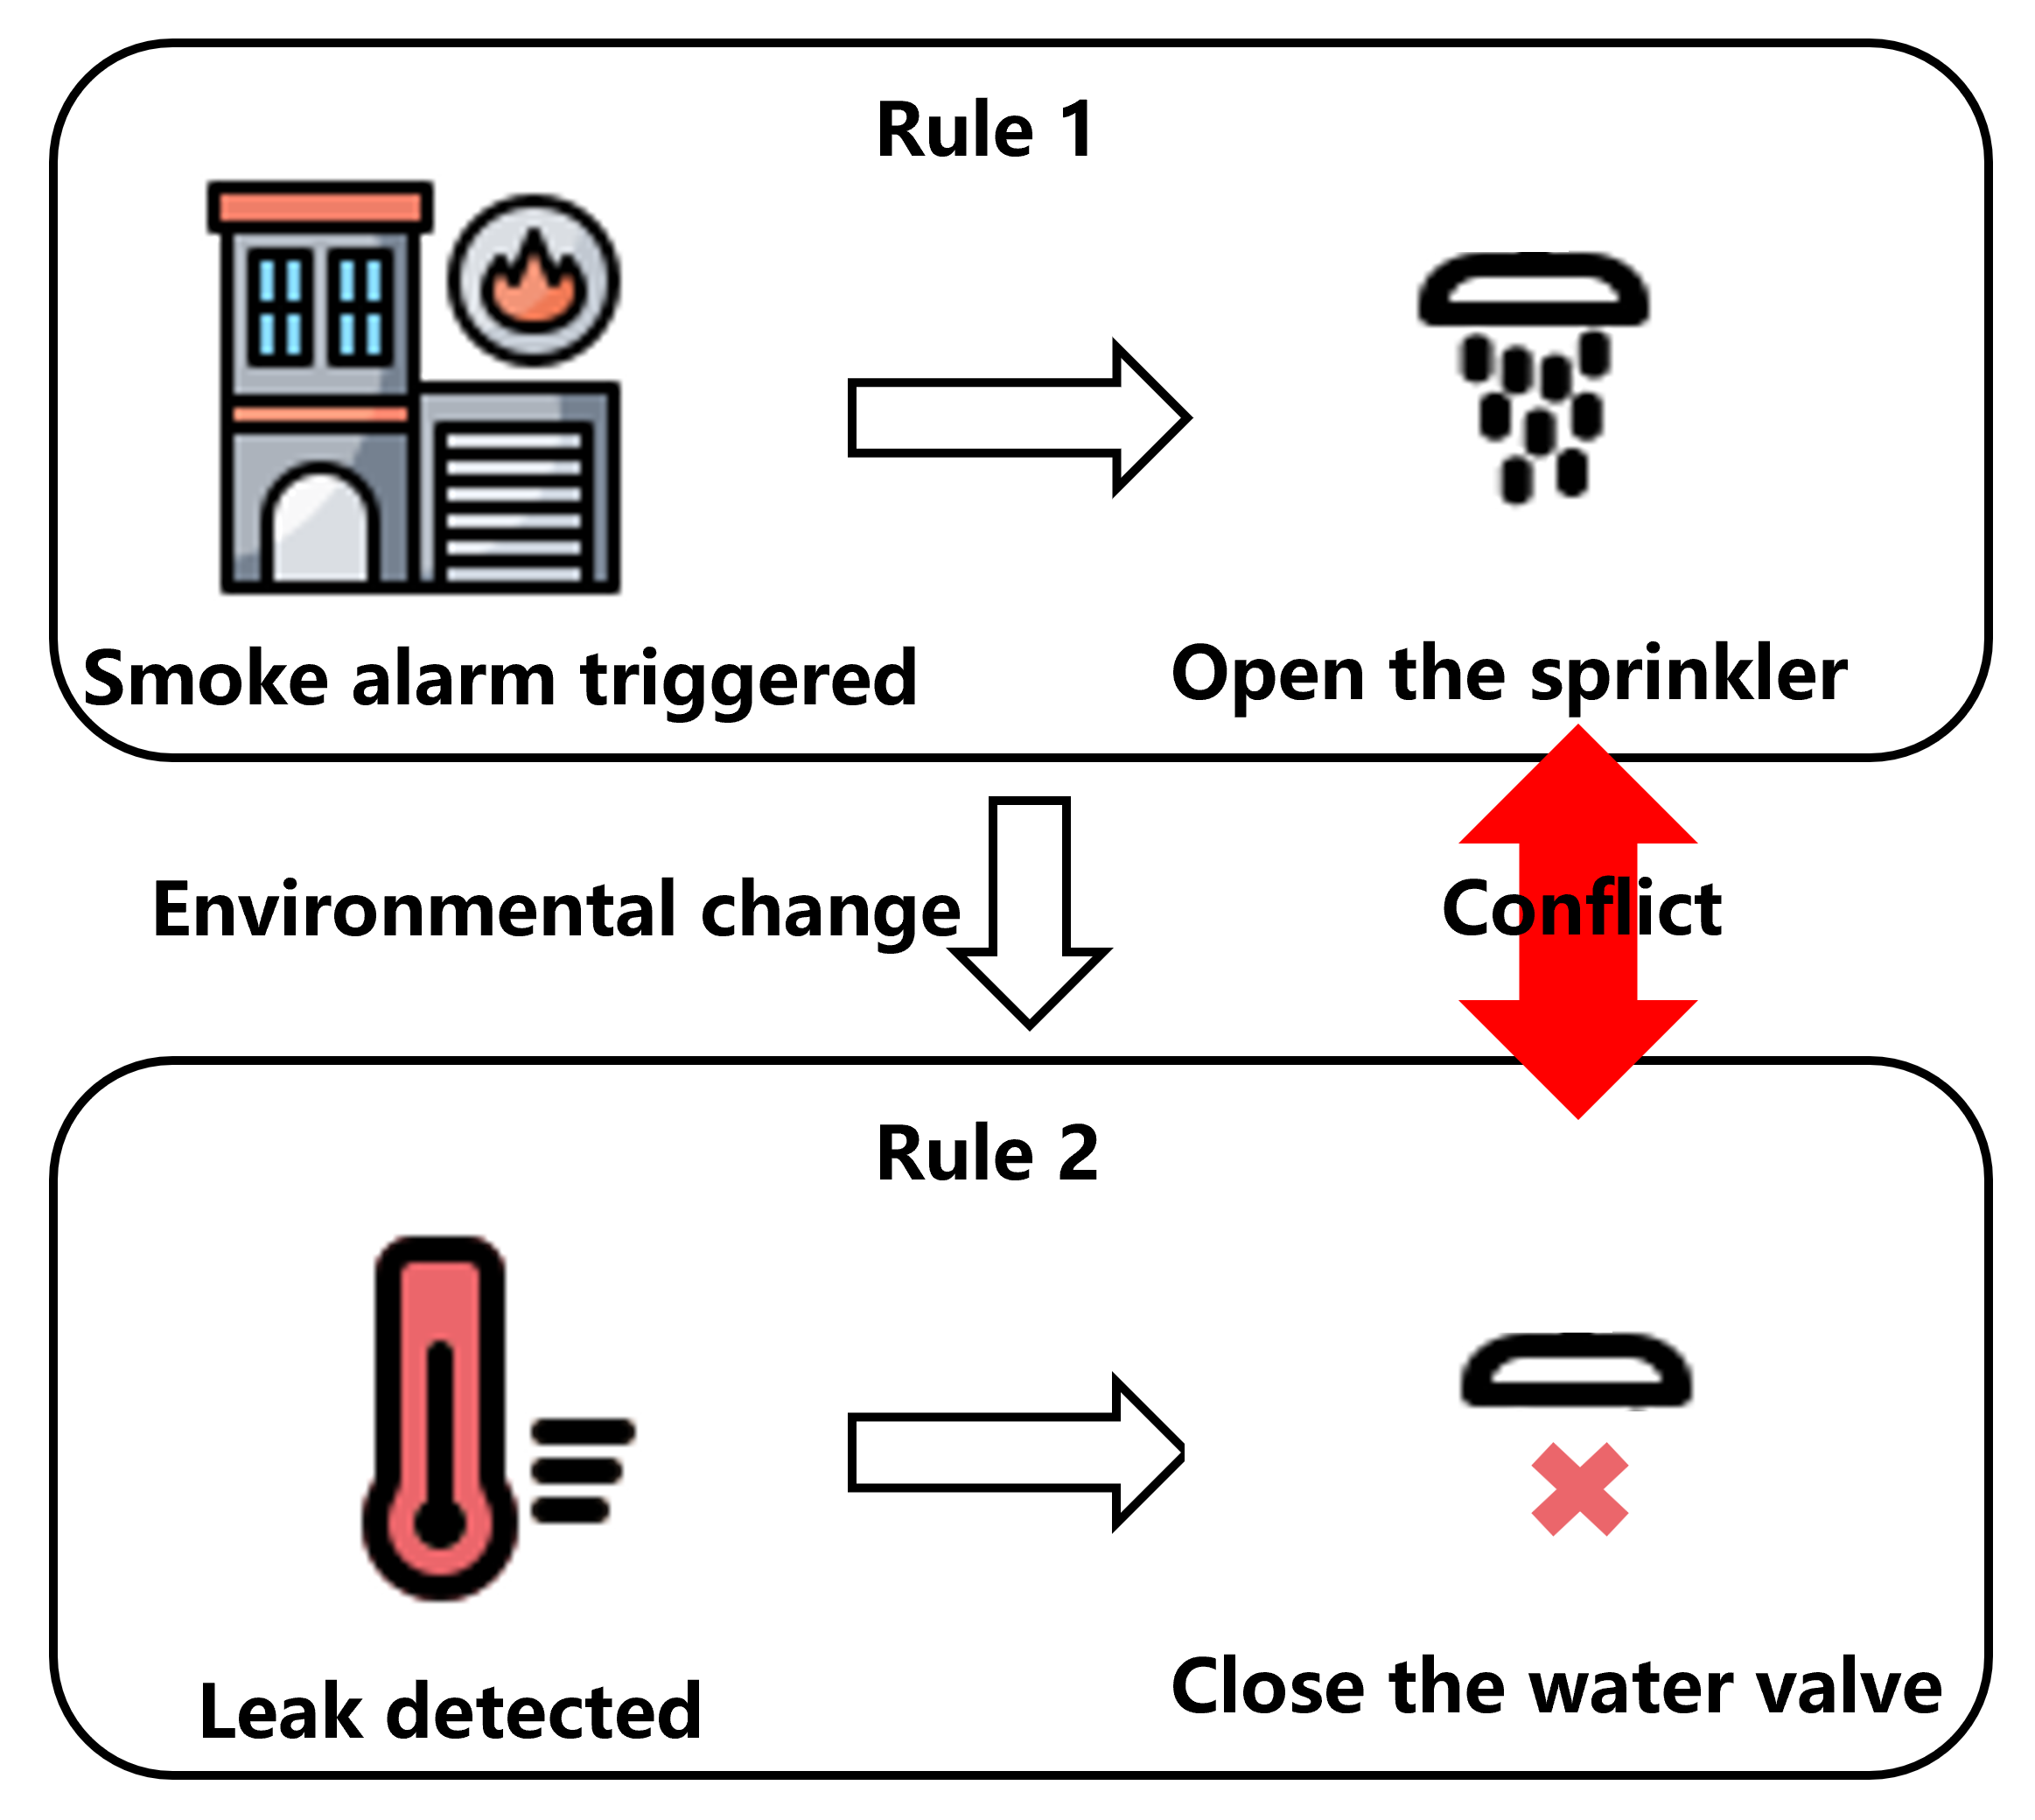
\includegraphics[width=0.4\textwidth]{figure/rule_conflict_example.png}
	\caption{Rule Conflict Example}
	\label{rule_conflict_example}
\end{figure}

% 针对智能家居中存在的规则冲突问题,目前已有一些研究致力于此。现有的规则冲突检测方法大致可以分为两类:(1)基于安全策略的方法:预先定义一套安全策略,若检测到当前规则的执行违反了这些策略,则判定为规则冲突;(2)基于规则交互模式的方法:根据规则之间的交互模式进行检测,若满足某种预定义的交互模式,则认为存在规则冲突的风险。
Several studies have addressed the issue of rule conflicts in smart homes\cite{alhanahnah2020scalable,chen2019multi,chi2020cross,ding2021iotsafe,huang2021conflict,li2020diac,xiao2019a3id,nakamura2005feature,igaki2010modeling,ibrhim2020formal,pradeep2021automating,shehata2007using,sun2014conflict,alharithi2019detecting,celik2019iotguard,hamza2022hsas,leelaprute2008detecting,trimananda2020understanding,yagita2015application,yu2022tapinspector,chaki2020fine,chi2023detecting,celik2018soteria,alhanahnah2022iotcom,ding2018safety,hsu2019safechain,wang2019charting}. Existing rule conflict detection methods can be broadly categorized into two types: (1) Security policy-based methods: A set of security policies is pre-defined, and any rule execution that violates these policies is flagged as a conflict\cite{celik2018soteria,celik2019iotguard,ding2021iotsafe}. (2) Rule interaction pattern-based methods: Detection is based on the interaction patterns between rules, and if a pre-defined interaction pattern is matched, a potential rule conflict is identified\cite{chi2020cross,chi2023detecting,celik2019iotguard,alhanahnah2022iotcom}.

% 规则冲突的处理方法主要有以下三种:(1)重新配置规则:修改或调整已有的规则,以消除冲突。(2)设置安全策略:定义特定的安全策略,确保即使发生规则冲突,执行结果也不会违反这些策略。(3)定制处理方法:针对特定的规则冲突,预定义专门的处理策略。这种方法可以看作是安全策略的扩展,为不同的冲突提供更精细化的解决方案。
Rule conflict resolution methods are mainly divided into the following three categories: (1) Rule reconfiguration: Existing rules are modified or adjusted to eliminate conflicts\cite{celik2018soteria,chen2019multi,chi2020cross,ding2018safety,hsu2019safechain,wang2019charting}. (2) Security policy enforcement\cite{celik2019iotguard,ding2021iotsafe}: Specific security policies are defined to ensure that execution results do not violate these policies, even if rule conflicts occur. (3) Custom resolution methods\cite{chi2023detecting}: Dedicated resolution strategies are pre-defined for specific rule conflicts. This approach can be viewed as an extension of security policies, providing more fine-grained solutions for different conflicts.

% 虽然现有的规则冲突解决方案在一定程度上缓解了该问题,但仍然存在一些局限性。
While existing rule conflict resolution schemes alleviate the problem to some extent, they still have certain limitations.

% 在规则冲突检测方面存在以下问题
The following issues exist regarding rule conflict detection.
\begin{itemize}
	% \item 依赖预定义的策略进行冲突检测的方法,无法覆盖所有可能的冲突场景。智能家居系统具有高度的个性化,通用的安全策略难以适用于所有家庭。例如,对于“检测到烟雾时开启喷淋”的规则,在某些家庭适用,但在另一些家庭可能不适用(例如,只希望在确认有明火时才开启喷淋)。不完备的安全策略会导致部分规则冲突无法被检测到。
	\item Detection methods\cite{celik2018soteria,celik2019iotguard,ding2021iotsafe} that rely on pre-defined policies for conflict detection cannot cover all possible conflict scenarios. Smart home systems are highly personalized, and generic security policies are difficult to apply to all households. For example, the rule "open the sprinkler when smoke is detected" may be appropriate in some homes, but not in others (e.g., only wanting to open the sprinkler when open flames are confirmed). Incomplete security policies can lead to the failure to detect some rule conflicts.
	
	% \item 基于规则交互模式的检测方法,容易产生误报。规则交互本身并不等同于规则冲突,其有效性高度依赖于具体的应用环境和用户偏好。例如,“日落时开启暖气”和“温度达到30\celsius时打开窗户并关闭暖气”这两条规则,在室内花园中可能是合理的,但在卧室中可能会导致能源浪费或不适。
	\item Detection methods\cite{chi2020cross,chi2023detecting,celik2019iotguard,alhanahnah2022iotcom} based on rule interaction patterns are prone to false positives. Rule interaction itself is not equivalent to a rule conflict, and its validity is highly dependent on the specific application environment and user preferences. For example, the rules "turn on the heating at sunset" and "open the window and turn off the heating when the temperature reaches 30\celsius" may be reasonable in an indoor garden, but could lead to energy waste or discomfort in a bedroom.
\end{itemize}

% 在规则冲突处理方面存在以下问题:
The following issues exist regarding rule conflict resolution.
\begin{itemize}
	% \item 直接修改规则配置可能会导致规则失效或引入新的冲突。简单地修改现有规则并不能保证完全解决问题,反而可能带来新的问题。
	\item Directly modifying rule configurations may cause the rules to malfunction or introduce new conflicts. Simply modifying existing rules does not guarantee a complete solution and may introduce new problems\cite{celik2018soteria,chen2019multi,chi2020cross,ding2018safety,hsu2019safechain,wang2019charting}.
	
	% \item  采用通用的安全策略,虽然可以在一定程度上保障家居安全,但缺乏个性化,无法满足不同用户的需求。
	\item While enforcing generic security policies can provide a certain level of home security, they lack personalization and cannot meet the needs of different users\cite{celik2019iotguard,ding2021iotsafe}.
\end{itemize}

\begin{figure}[htbp]
	\centering
	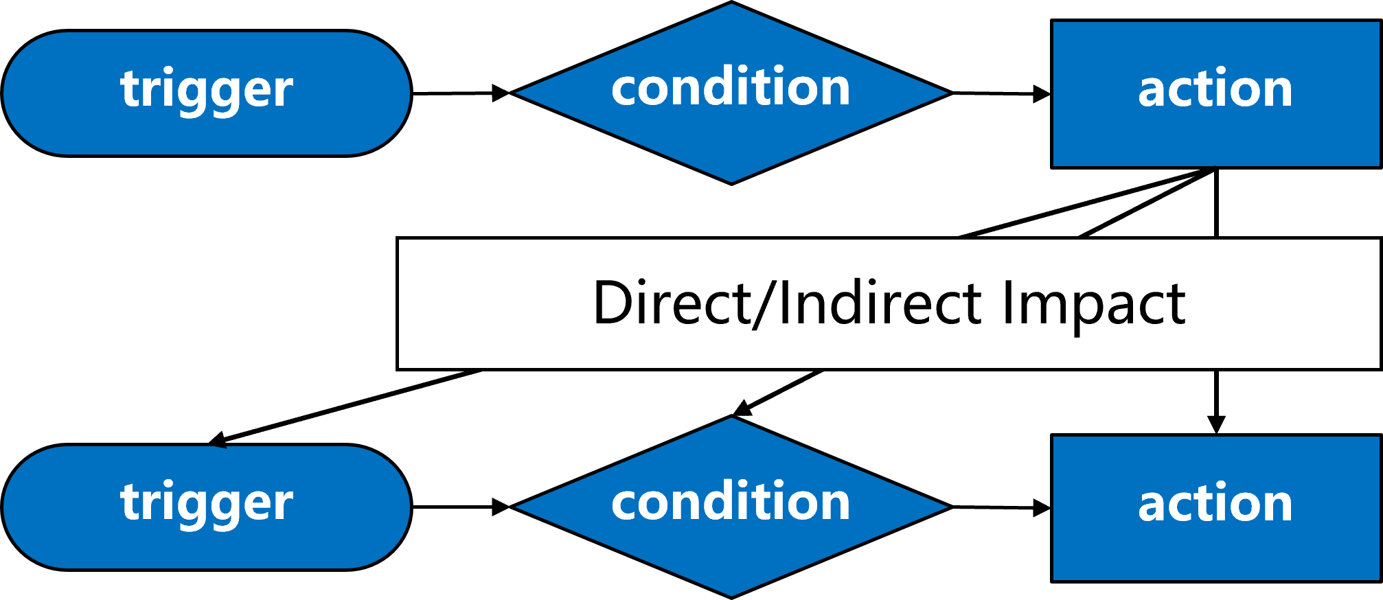
\includegraphics[width=0.4\textwidth]{figure/classification_observation.png}
	\caption{Rule Interaction Pattern}
	\label{classification_observation}
\end{figure}

% 为了解决这些问题,本研究基于以下观察:(1)规则可以使用TCA表示,一条规则可能对另一条规则的触发器、条件和动作产生直接或者间接影响,因此规则之间的交互可以归纳为六种类型 (如图 \ref{classification_observation}所示):一条规则的执行结果可能直接或间接地影响另一条规则的触发、条件或动作。(2)规则交互是否构成冲突是主观的,取决于用户的偏好。(3)智能家居系统通常采用TCA模型来执行规则,但是在规则冲突的检测与处理中还需要考虑到其他通道的影响,且具有区域特征,例如开放式厨房的布局下厨房的温度与湿度特征可能与客厅的温度与湿度特征相关联,而与卧室的温度与湿度特征往往不相关,因此需要对规则特征进行更多的信息采样。
To address these issues, this study is based on the following observations: (1) Rules can be represented using the TCA model, where one rule may directly or indirectly affect the trigger, condition, and action of another rule. Therefore, interactions between rules can be categorized into six types (as shown in \ref{classification_observation}): the execution result of one rule may directly or indirectly affect the trigger, condition, or action of another rule. (2) Whether rule interactions constitute conflicts is subjective and depends on user preferences. (3) Smart home systems typically use the TCA model to execute rules, but the detection and handling of rule conflicts require considering the influence of other channels and have regional characteristics. For example, in an open kitchen layout, the temperature and humidity characteristics of the kitchen may be related to those of the living room, but often unrelated to those of the bedroom. Therefore, more information sampling of rule features is needed.

% 基于以上观察,本文提出了一种新的规则冲突检测与解决方法。首先,我们基于规则交互模式对交互类型进行分类。为了捕获间接通道的影响,本研究通过结合用户环境配置来对规则重新建模,并使用形式化分析方法进行模型检查,以发现所有可能的规则交互。然后,我们结合实体的用户安全配置来实现基本的冲突检测和冲突解决方法策略建议。用户也可以根据自己的偏好进行调整。此外,本研究充分利用了智能家居系统基于TCA模型执行规则的事实,并且当发生规则冲突时,可以选择性地执行规则,从而为每对冲突规则实现定制化的解决方法策略,而不是采用一刀切的通用安全策略。
Based on the above observations, this paper proposes a new rule conflict detection and resolution method. First, we classify interaction types based on rule interaction patterns. To capture the impact of indirect channels, this study re-models rules by incorporating user environment configurations and uses formal analysis methods for model checking to discover all possible rule interactions. Then, we combine the user's security configurations for entities to implement basic conflict detection and conflict resolution strategy recommendations. Users can also make adjustments according to their own preferences. Furthermore, this study takes full advantage of the fact that smart home systems execute rules based on the TCA model, and when rule conflicts occur, rules can be selectively executed, thereby enabling customized resolution strategies for each pair of conflicting rules, rather than adopting a one-size-fits-all general security policy.

% 总而言之,我们的贡献如下:
In summary, we make the following contributions:

\begin{itemize}
	% \item 我们提出了一种基于规则执行机制的规则冲突分类方法,该方法涵盖了所有规则交互类型。
	\item We propose a rule conflict classification method based on the rule execution mechanism that covers all rule interaction types.
	
	% \item 我们设计并实现了一种结合静态和动态冲突检测的方案,适用于智能家居规则的广泛冲突检测机制:通过为规则增加区域属性并重新建模,结合安全实体配置进行静态冲突检测;同时,采用断言检测的方法在运行时检测系统中是否存在规则冲突。
	\item We design and implement a solution combining static and dynamic conflict detection to achieve a widely applicable conflict detection mechanism suitable for smart home rules: Static conflict detection is performed by adding region attributes to the rules and remodeling them, combined with security entity configuration; at the same time, assertion detection methods are used to detect whether rule conflicts exist in the system during runtime.
	
	% \item 我们设计并实现了冲突解决方案、定制化的冲突规则处理策略以及冲突预防措施:基于规则执行机制,实现了多种冲突处理策略,并根据安全实体配置自动选择合适的处理策略。此外,还可以在规则冲突发生前进行拦截,以防止冲突发生。
	\item We design and implement conflict resolution solutions, customized conflict rule resolution strategies, and conflict prevention measures: Based on the rule execution mechanism, multiple conflict resolution strategies have been implemented, and appropriate resolution strategies are automatically selected based on security entity configuration. In addition, conflicts can be intercepted before they occur to prevent conflicts from occurring.
\end{itemize}
